\documentclass[10pt,a4paper]{article}

\usepackage[margin=2cm]{geometry}
\usepackage[T1]{fontenc}
\usepackage{lmodern}
\usepackage{amsmath,amssymb}
\usepackage{graphicx}
\usepackage{booktabs}
\usepackage{multirow}
\usepackage{subcaption}
\usepackage{xcolor}
\usepackage{enumitem}
\usepackage[hidelinks]{hyperref}

\setlist{itemsep=1pt,topsep=3pt}
\graphicspath{{figures/}}
\let\oldus\_
\renewcommand{\_}{\oldus\allowbreak}
\emergencystretch=2em
\setlength{\textfloatsep}{8pt}
\setlength{\floatsep}{6pt}
\setlength{\abovecaptionskip}{3pt}

\title{\vspace{-1.5cm}\textbf{Predicting Human Development Level from Economic Indicators}\\
\large DS203: Programming for Data Science, Group Project}
\author{\normalsize Vedant Iyengar (25B2141) \quad Rehan Mallik (25B0408)
  \quad Siddhartha Nair (25B3990)}
\date{\vspace{-0.6cm}}

\begin{document}
\maketitle

\section{Introduction}


The UNDP's Human Development Index (HDI) combines health, education
and economic statistics into one score, but it is published only yearly, sometimes with delays. The dataset is rough and has missing values for certain countries. World Bank indicators, on the other hand, are released more often and for more economies. If they can predict a country's HDI tier
(three classes, Low / Medium-High / Very High), they can give an early
estimate where the HDI is late or absent and show which measurable
characteristics are most closely associated with human development. We
compare a majority-class baseline, multinomial logistic regression, a
decision tree and a random forest, with and without PCA to test this very signal.


\section{Methodology}


\subsection{Dataset Download and Setup}

\paragraph{Data sources and merging.} We combined 2023 HDI scores from the \textbf{UNDP HDI} time series with 2023 development indicators and region codes from the \textbf{World Bank API} (\texttt{wbgapi}). Merging on country code gave 195 countries and automatically dropped regional aggregates and territories. Two of these countries (\texttt{MCO} and \texttt{PRK}) do not have a 2023 HDI score and are dropped before training. Where a 2023 World Bank value was missing, we used the most recent earlier year (2018--2022)---affecting 32 values across 19 countries, logged in \texttt{substituted\_years.csv}.

\paragraph{Target and feature engineering.} From the merged table, we grouped \texttt{hdi\_2023} into three target classes (\texttt{Level}): $< 0.550$ (Class~0, Low), $0.550\text{--}0.799$ (Class~1, Medium/High), and $\ge 0.800$ (Class~2, Very High). We also computed \texttt{Services} share ($100 - \text{Agriculture} - \text{Industry}$) and \texttt{Dominant\_Sector} (the sector with the largest GDP share). Full column definitions and sources are in \texttt{Data\_Dictionary.md}.

\subsection{Exploratory Data Analysis}
\label{sec:eda}

\paragraph{Dataset overview.} The dataset covers 195 countries across 14
columns, including 10 numerical predictors, 2 categorical predictors, 1
country identifier, and the target variable \texttt{Level}. Most of the
processes followed during EDA were derived with the help of the lecture
notebook on the same.

\paragraph{Missing value patterns.} \texttt{Region} and
\texttt{Access\_to\_electricity} have no missing values. In other places, gaps are
concentrated in the lowest HDI class, which was a recurring pattern across
our dataset. However, it is not universal; \texttt{Unemployment\_total} is
fully reported in Class 0.0 but missing in 8.6\% of Class 1.0 and 8.1\% of
Class 2.0 countries. Since missingness is therefore not completely at random,
we impute with training-set medians and add a binary missing-value indicator
for each numerical feature, so that the information carried by a gap is not
lost.

\paragraph{Patterns across HDI classes \& feature correlations.} We found
several correlations while analysing the indicators (Fig.~\ref{fig:eda}b),
implying that not all of them are fully independent.
\texttt{Individuals\_using\_the\_Internet} and \texttt{Infant\_mortality}
show clear separation across classes. \texttt{Agriculture} decreases with
HDI, while \texttt{Services} increases. \texttt{Industry},
\texttt{Inflation\_consumer\_prices}, \texttt{Unemployment\_total}, and
\texttt{GDP\_Growth} overlap considerably. These positive and negative
correlations make intuitive sense and thus reinforce the validity of the
dataset.

\paragraph{Categorical feature analysis.} Every labelled country has a World
Bank region code, and HDI classes split clearly across regions
(Fig.~\ref{fig:eda}a). \texttt{EAS}, \texttt{LCN} and \texttt{SAS} are mostly
Class 1 with no Class 0 countries, while \texttt{ECS} (86.3\%) and
\texttt{NAC} (100\%) are concentrated in Class 2. \texttt{MEA} is spread
across all three tiers, whereas \texttt{SSF} holds 22 of the 26 Class 0
countries. Services is the dominant sector in 177 out of 193 labelled
countries; the Industry (8) and Agriculture (2) groups are too small to read
much into, so the continuous sector-share columns carry this information
better.

\begin{figure}[h]
  \centering
  \begin{subfigure}[b]{0.49\linewidth}
    \centering
    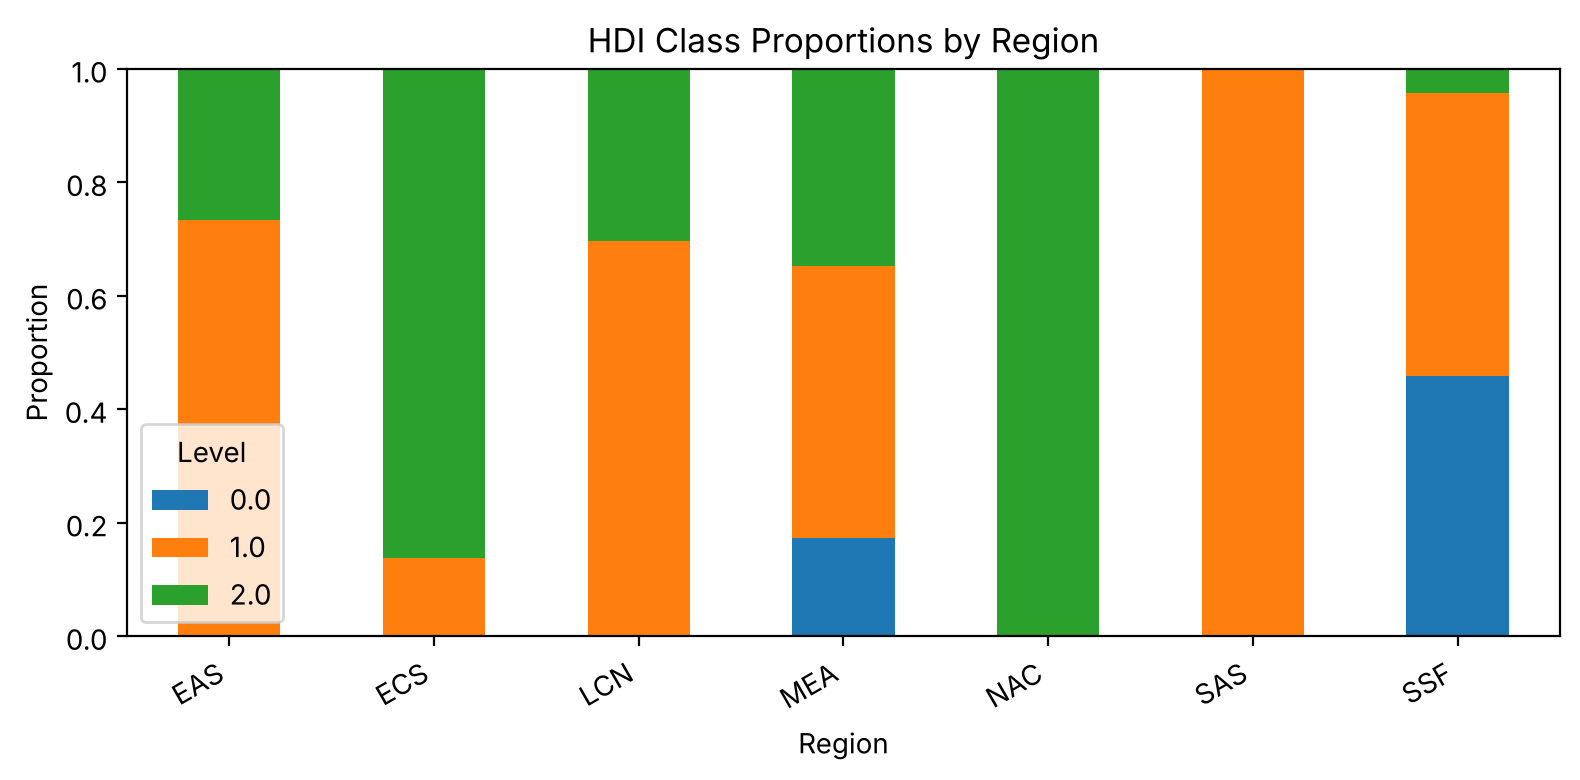
\includegraphics[width=\linewidth]{region_by_class.png}
    \caption{Class proportions by region.}
  \end{subfigure}\hfill
  \begin{subfigure}[b]{0.42\linewidth}
    \centering
    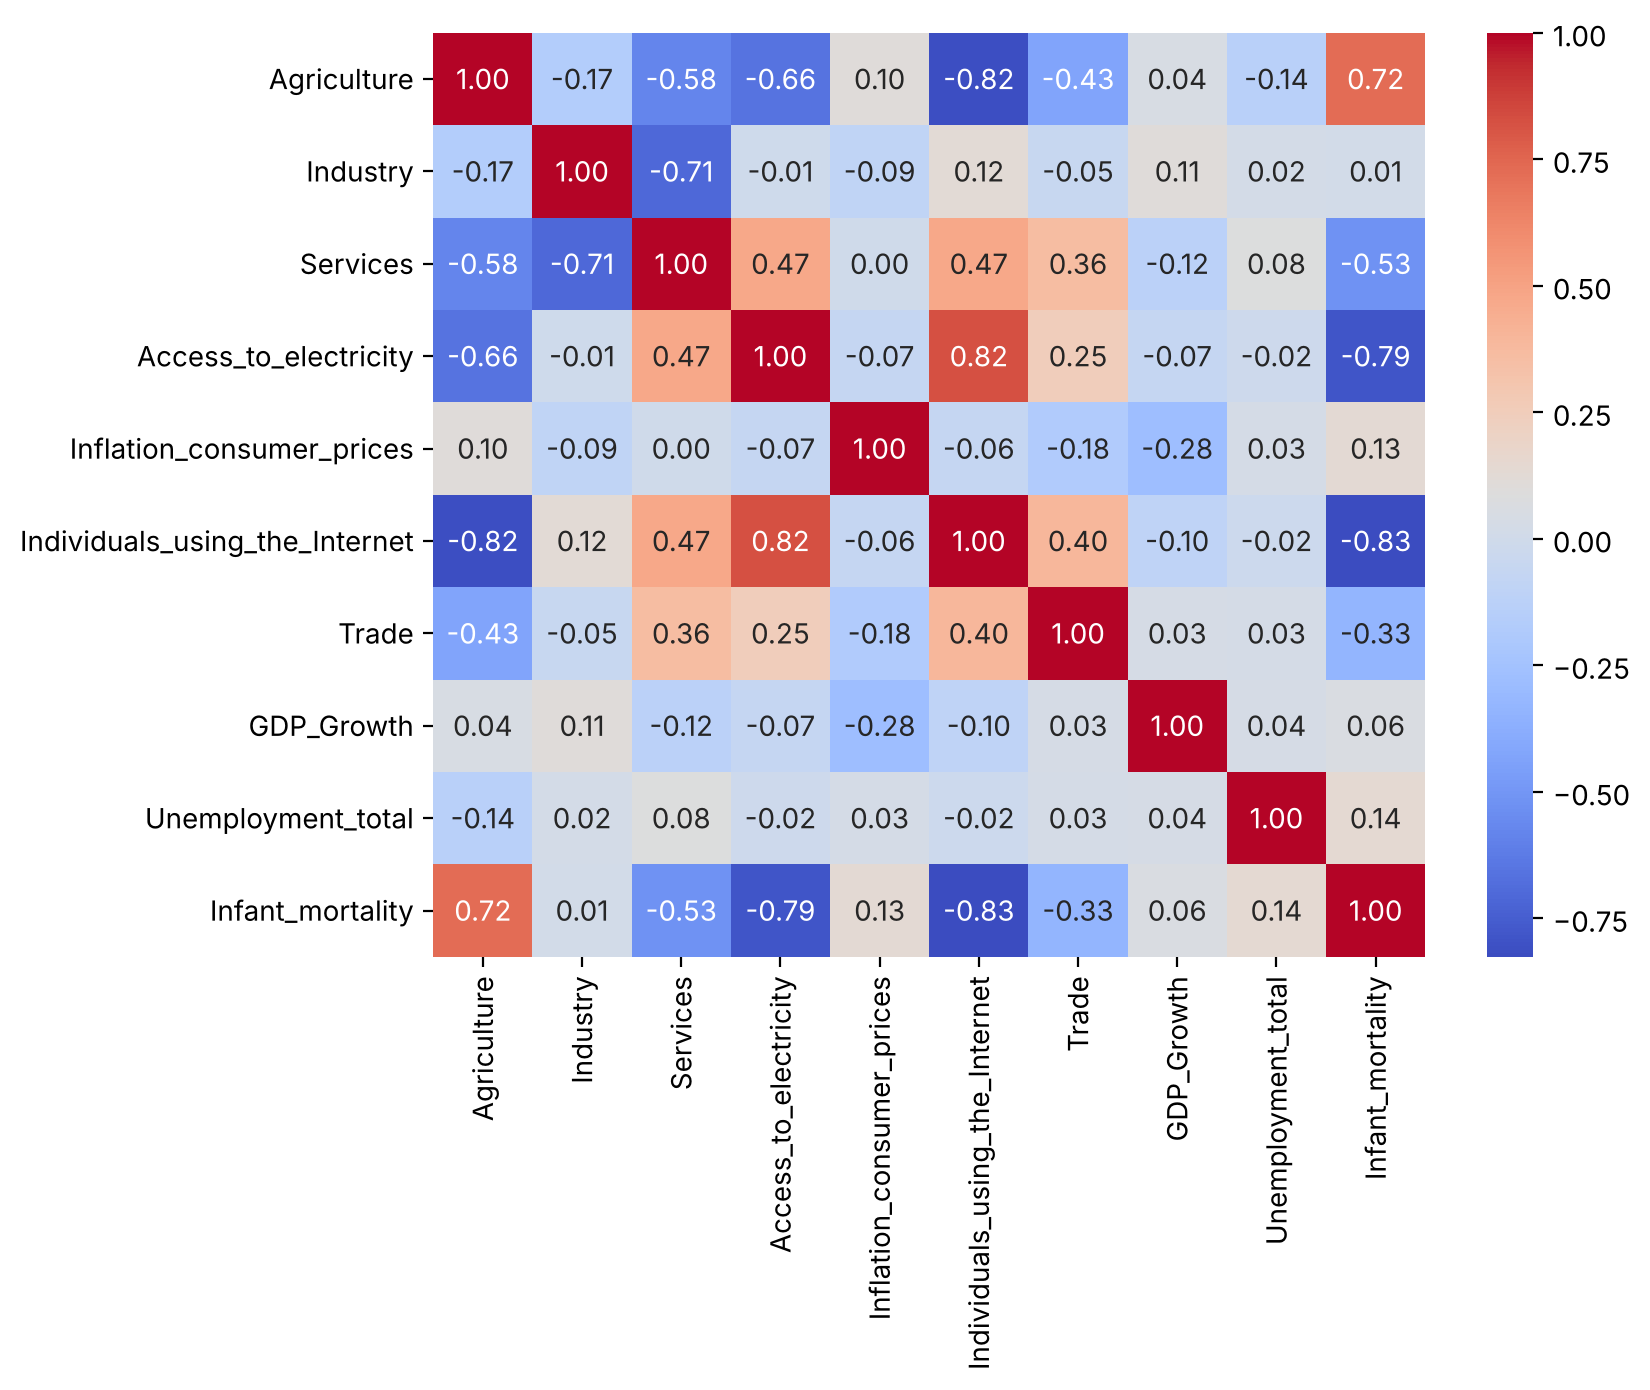
\includegraphics[width=\linewidth]{correlation_heatmap.png}
    \caption{Correlation of numerical features.}
  \end{subfigure}
  \caption{Exploratory analysis.}
  \label{fig:eda}
\end{figure}

\subsection{Preprocessing}

\begin{itemize}[leftmargin=*]
  \item \textbf{Split:} Removing rows where HDI is NaN. Dropping country
        name (it does not serve as a predictor). Splitting data into
        test/train/validation (stratified split i.e.\ roughly each class
        appears in the same amount in each split): 60/20/20, i.e.\
        115/39/39 countries, \texttt{random\_state=10}.
  \item \textbf{Numerical imputation:} Compared to mean imputation, median
        imputation is more resistant to outliers. As such we went with
        median imputation (our data has many outliers); we found medians
        w.r.t.\ train set. But, it is possible that a value being missing is
        important information to predict the HDI; to account for this
        possibility, we are adding missing indicators (\texttt{add\_indicator=True}),
        i.e.\ for numerical columns with missing values, we are adding
        another column where each missing value gets a `1' and rest of the
        rows are `0'.
  \item \textbf{Categorical encoding:} Missing \texttt{Dominant\_Sector}
        values (and any missing \texttt{Region}) are filled with
        ``missing'' and one-hot encoded using
        \texttt{OneHotEncoder(handle\_unknown="ignore")} (dealing with unseen
        categories). This gives 30 columns in total.
  \item \textbf{Scaling:} \texttt{StandardScaler} on the original numerical
        columns in a \texttt{ColumnTransformer} inside a \texttt{Pipeline};
        it doesn't scale binary values.
  \item \textbf{PCA:} Fit on the training set only, checking cumulative
        explained variance against a 90\% threshold. We compared the accuracy
        score of no PCA vs different numbers of components (1 to 12) using
        PCA. To calculate the accuracy score we used LR, Decision Tree, and
        Random Forest, fit them on the training set and predicted on the
        validation set.
\end{itemize}

\subsection{Models and Evaluation}

All models are trained on the PCA components of the training set
(\texttt{PCA(n\_components=0.9)}, keeping 8 components).
\begin{itemize}[leftmargin=*]
  \item \textbf{Majority-class baseline:} always predicts the most common
        class in the training set (Class 1.0). Any useful model has to beat
        this.
  \item \textbf{Multinomial logistic regression (LR):} \texttt{random\_state=10},
        tuned over $C \in \{0.01, 0.1, 1.0, 10.0\}$ (selecting $C=1$).
  \item \textbf{Decision tree} and \textbf{random forest (RF):} both use
        \texttt{random\_state=10}; decision tree is tuned over
        $\texttt{max\_depth} \in \{1, 3, 7, \text{None}\}$ (selecting $3$),
        and RF is tuned over $\texttt{n\_estimators} \in \{50, 100, 200\}$
        (selecting $200$).
\end{itemize}

\noindent The classes are imbalanced (13\% / 48\% / 38\%), so a model can get
almost 50\% accuracy by ignoring Class 0.0 entirely. Hence \textbf{macro F1}
is our main metric; accuracy and balanced accuracy are also reported. Models
are compared on the validation set and tuned with 5-fold stratified
cross-validation (\texttt{StratifiedKFold}, \texttt{random\_state=10}) on
the train+validation countries, where imputation, encoding, scaling and PCA
are refit inside a \texttt{Pipeline} in every fold so no information leaks
from the held-out part. We also check LR validation macro F1 across feature
subsets (numerical-only, categorical-only, and without region or dominant
sector) and compute test-set permutation importance (30 shuffles). The test
set is used only once, at the very end.
\section{Experiments}

\subsection{Preprocessing and PCA}

The class count percentages are approximately the same across train, test
and validation sets. To inspect how much variance each component captures,
we have plotted the individual and cumulative explained variance after PCA on
the training set (Fig.~\ref{fig:pca}a). The first two components alone
explain about 49\% of the variance. Table~\ref{tab:loadings} shows the top
features contributing to each component: PC1 is built from internet users,
infant mortality and agriculture, the living-condition indicators that
separated the classes in EDA, whereas PC2 is built from GDP growth,
inflation and industry.

\noindent Eight components pass the 90\% variance threshold. Validation
accuracy (LR) rises to 0.85 across 5 to 9 components and then drops to 0.79
at 10 components (Fig.~\ref{fig:pca}b), so the extra components mostly add
noise. Without PCA, the same LR on all 30 columns scores only 0.79. N=8
therefore sits on the plateau while crossing the 90\% variance line with
fewer components.

\begin{figure}[h]
  \centering
  \begin{subfigure}[b]{0.4\linewidth}
    \centering
    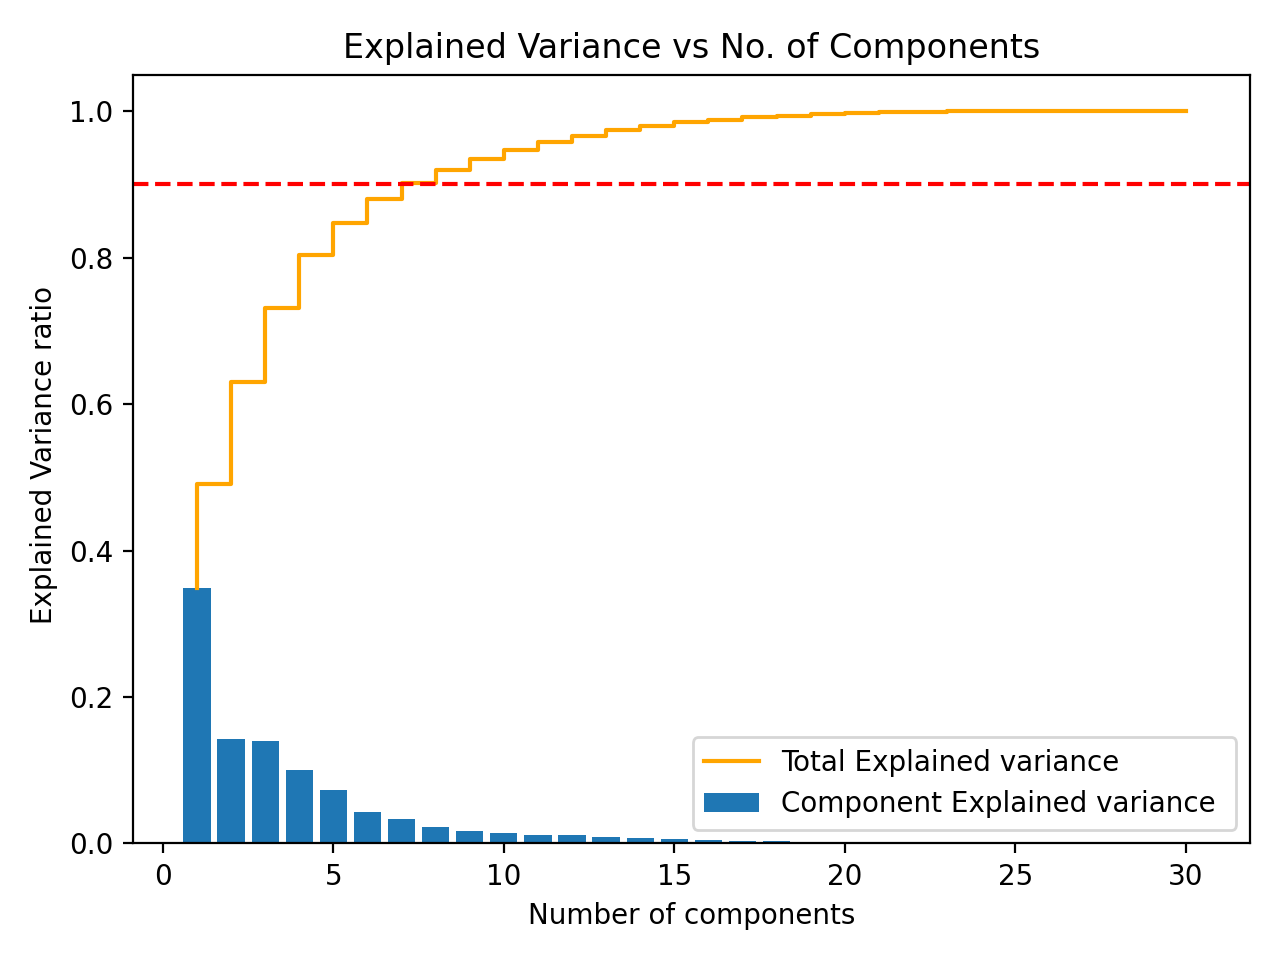
\includegraphics[width=\linewidth]{pca_variance.png}
    \caption{Explained variance vs components.}
  \end{subfigure}\hspace{1em}
  \begin{subfigure}[b]{0.4\linewidth}
    \centering
    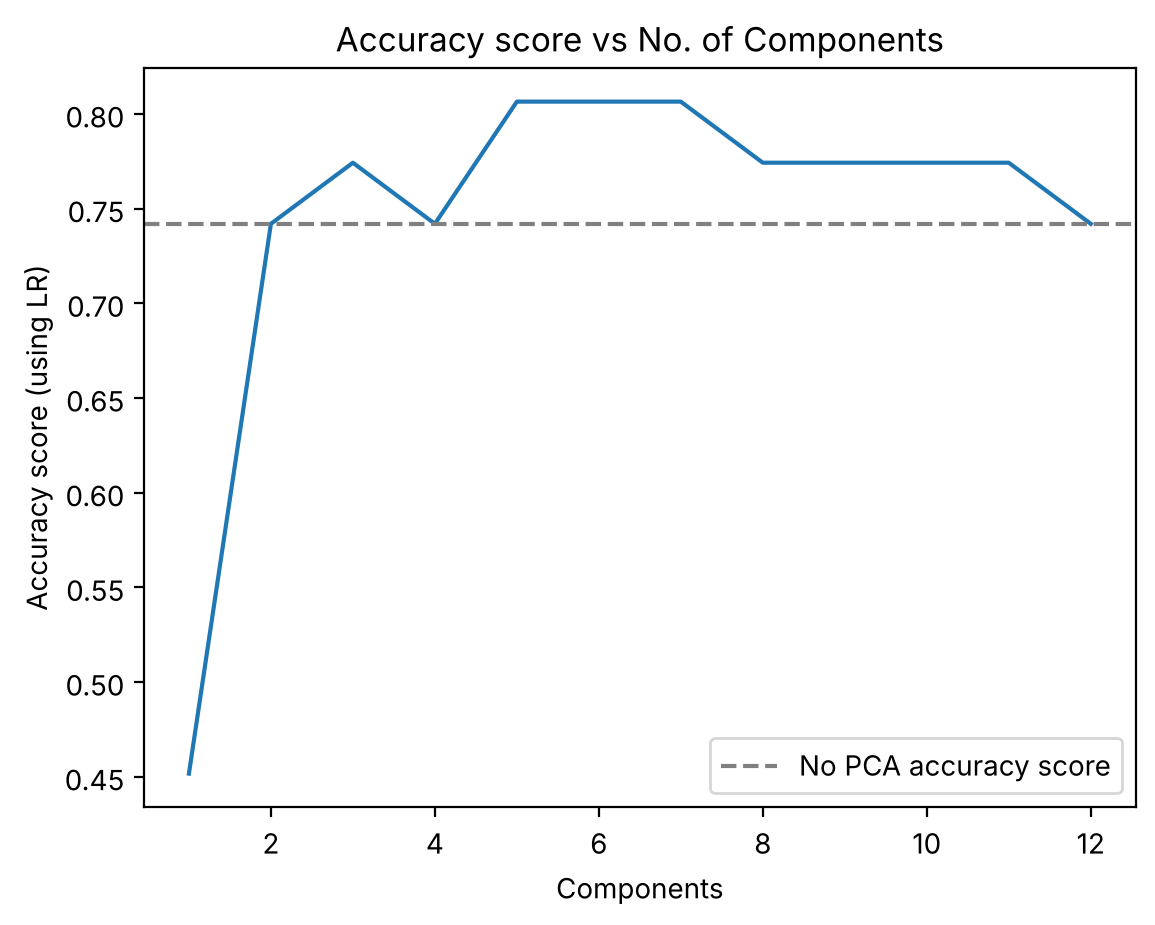
\includegraphics[width=\linewidth]{pca_accuracy.png}
    \caption{Validation accuracy (LR) vs components.}
  \end{subfigure}
  \caption{PCA on the training set.}
  \label{fig:pca}
\end{figure}

\begin{table}[h]
\centering
\footnotesize
\caption{Top 3 features which contributed the most to each component
(by absolute loading).}
\label{tab:loadings}
\begin{tabular}{@{}llll@{}}
\toprule
PC1 & PC2 & PC3 & PC4 \\
\midrule
Internet & GDP growth & Industry & Unemployment \\
Infant mortality & Inflation & Services & Agriculture \\
Agriculture & Industry & Inflation & Infant mortality \\
\bottomrule
\end{tabular}
\end{table}
\subsection{Model Comparison}

\begin{table}[h]
\centering
\footnotesize
\caption{Results. Validation and CV use macro F1 (CV: mean $\pm$ std over 5
folds). Test set: 39 countries.}
\label{tab:results}
\begin{tabular}{@{}lccccc@{}}
\toprule
& \multicolumn{2}{c}{Model selection} & \multicolumn{3}{c}{Test set} \\
\cmidrule(lr){2-3}\cmidrule(l){4-6}
Model & Val.\ F1 & CV F1 & Accuracy & Bal.\ accuracy & Macro F1 \\
\midrule
Majority baseline   & 0.22 & --                    & 0.49 & 0.33 & 0.22 \\
Logistic regression & \textbf{0.86} & \textbf{0.80 $\pm$ 0.07} & \textbf{0.95} & \textbf{0.96} & \textbf{0.96} \\
Decision tree       & 0.72 & 0.71 $\pm$ 0.13 & 0.90 & 0.92 & 0.90 \\
Random forest       & 0.84 & 0.76 $\pm$ 0.05 & \textbf{0.95} & 0.91 & 0.94 \\
\bottomrule
\end{tabular}
\end{table}

\paragraph{Selection.} All three models beat the baseline by a wide margin
(Table~\ref{tab:results}). LR has the best validation F1 and the best CV F1,
so we picked it as our final model. On the test set RF matches LR on
accuracy (0.95) and comes close on macro F1 (0.94 vs.\ 0.96), missing just
one Class 0.0 country that LR gets right. The decision tree is the least
stable: its CV score varies most across folds (std 0.13) and it drops to
0.90 on the test set, the usual sign of a single tree overfitting. Tuning
\texttt{n\_estimators} over $\{50, 100, 200\}$ for RF picked 200 trees
(0.76 CV F1).

\paragraph{Errors.} LR places 37 of 39 test countries correctly
(Fig.~\ref{fig:results}a). Both mistakes are one class away and lie close
to the 0.80 cut-off: Moldova (HDI 0.785, Class 1.0 predicted as 2.0) and
Trinidad and Tobago (0.807, 2.0 predicted as 1.0). Countries far from a
boundary are never confused.

\paragraph{What the models relied on.} Permutation importance (drop in test
macro F1 when one original indicator is shuffled, 30 repeats) puts
\texttt{Access\_to\_electricity} first (0.25 for LR, 0.16 for RF), followed
by \texttt{Agriculture} (0.15), \texttt{Individuals\_using\_the\_Internet}
(0.14) and \texttt{Infant\_mortality} (0.14) (Fig.~\ref{fig:results}b); RF
has the same top four. On the validation set, LR trained on the numerical
features alone reaches a macro F1 of 0.81, against 0.64 for the categorical
features alone and 0.86 for both. Dropping \texttt{Region} or
\texttt{Dominant\_Sector} leaves validation F1 at 0.86, so the continuous
indicators carry most of the signal while the categorical columns add a
small boost over numerical features alone.

\begin{figure}[h]
  \centering
  \begin{subfigure}[b]{0.36\linewidth}
    \centering
    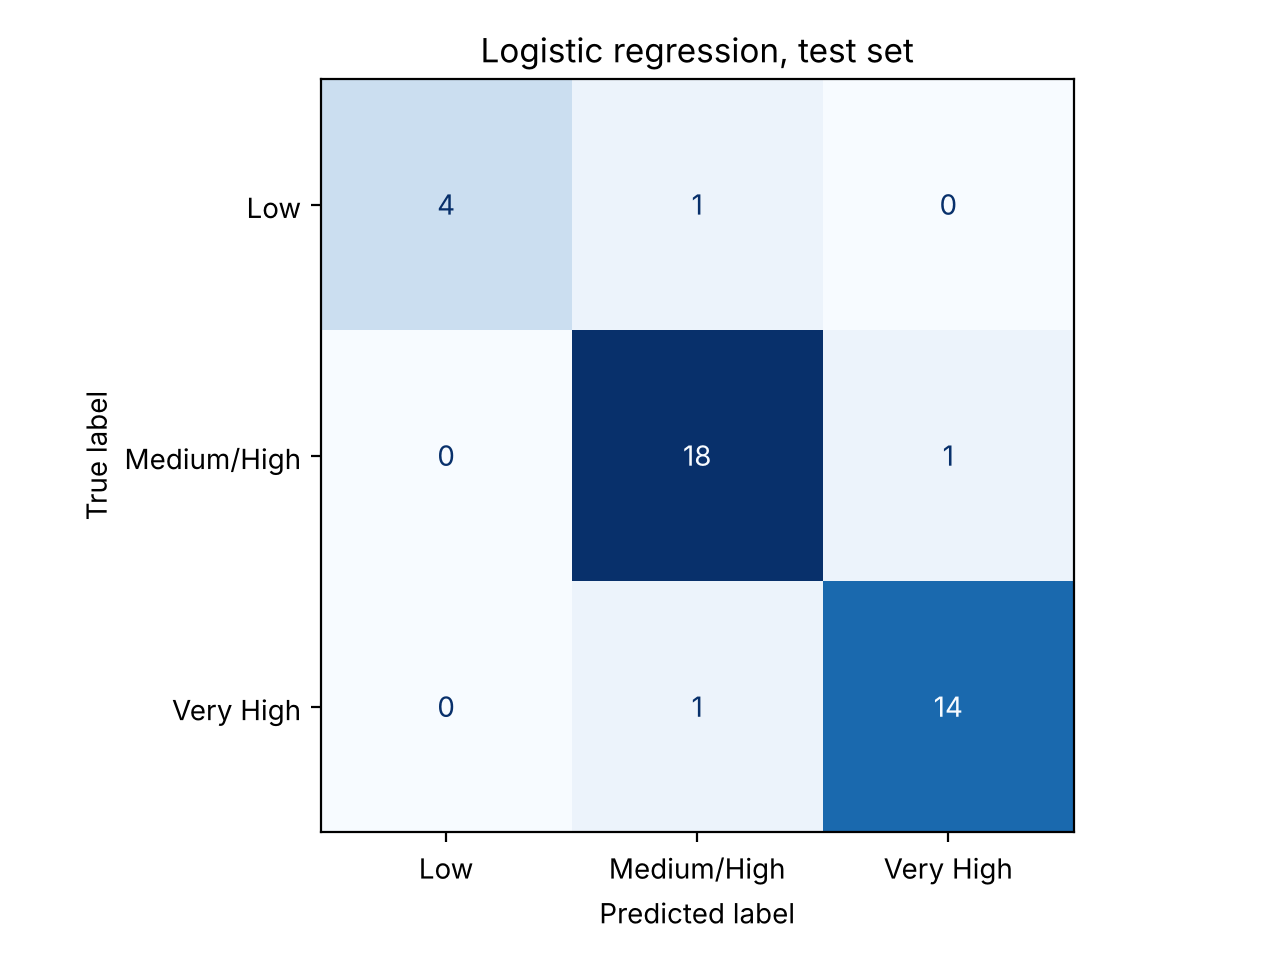
\includegraphics[width=\linewidth]{confusion_matrix.png}
    \caption{Confusion matrix, LR, test set.}
  \end{subfigure}\hspace{1em}
  \begin{subfigure}[b]{0.5\linewidth}
    \centering
    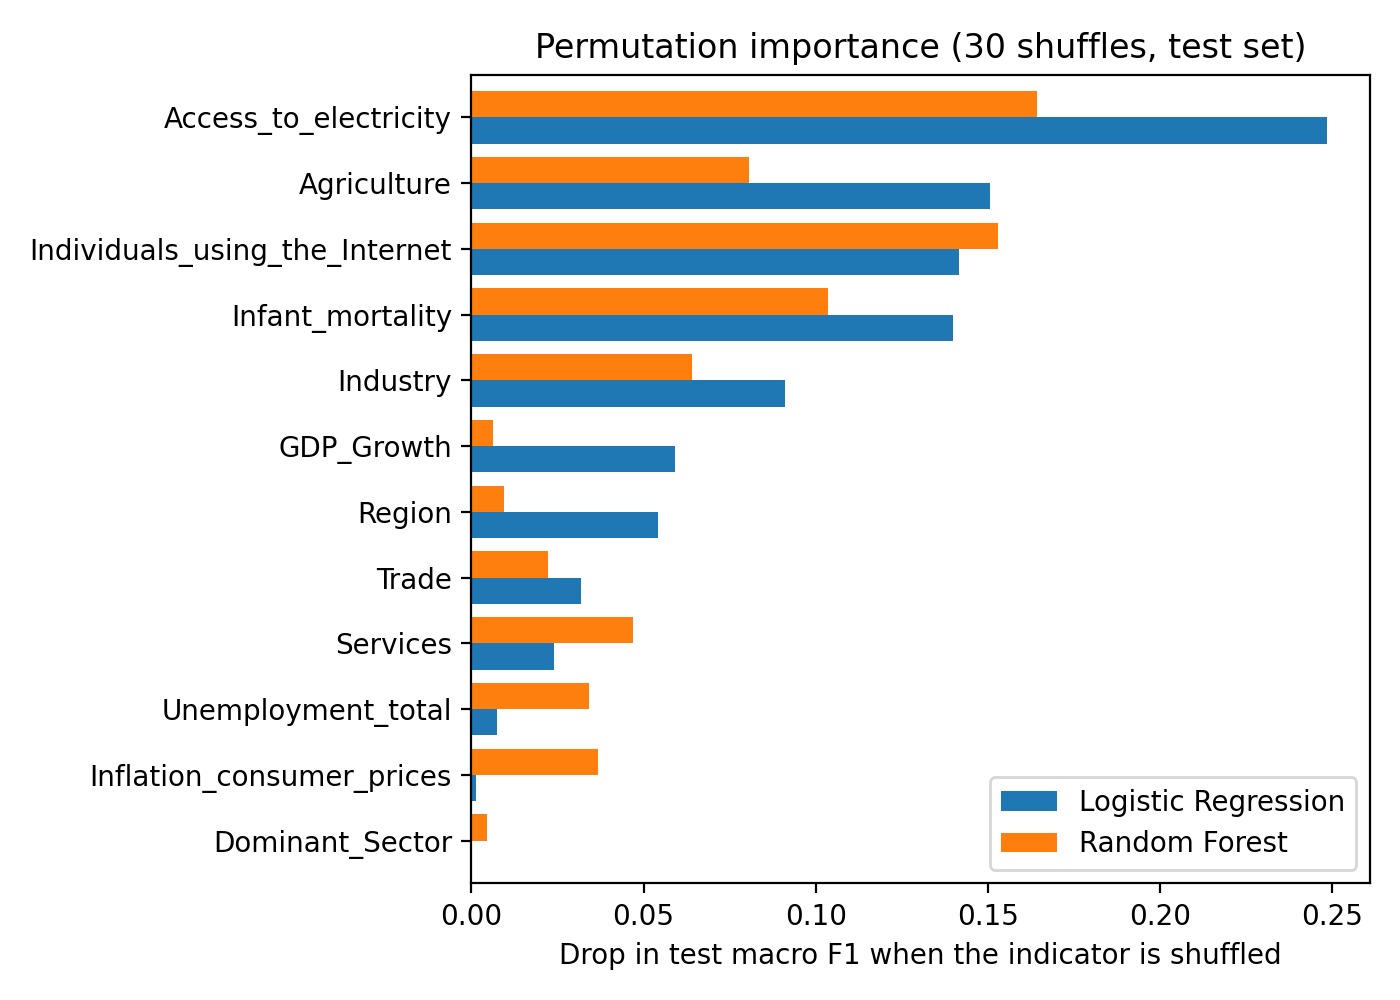
\includegraphics[width=\linewidth]{perm_importance.png}
    \caption{Permutation importance, test set.}
  \end{subfigure}
  \caption{Final evaluation.}
  \label{fig:results}
\end{figure}
\subsection{Discussion and Conclusion}

World Bank indicators can predict a country's HDI tier well: our final
model, a multinomial logistic regression on eight PCA components, classifies
95\% of unseen countries correctly (macro F1 0.96), against 49\% for the
baseline. Most of the signal comes from a few living-condition indicators
(electricity, internet use, farming share and infant mortality), which
matches the class separation we saw in EDA. Growth, inflation and
unemployment contribute little. The simplest model did best, which suggests
the classes are close to linearly separable once the data is scaled and
reduced.

\paragraph{Limitations.} These are associations, not causes: more internet
access would not by itself raise a country's HDI. We use one year and 193 countries, so the test set is small and one country moves accuracy by
2.6 points. The three classes and their cut-offs are our own choice, and
countries near a cut-off are exactly where the model fails. PCA also makes
the model harder to interpret directly, which is why we measured importance
on the original indicators.
\end{document}